\section{System Overview}
\label{sec-system-overview} 
\begin{figure}
    \centering
       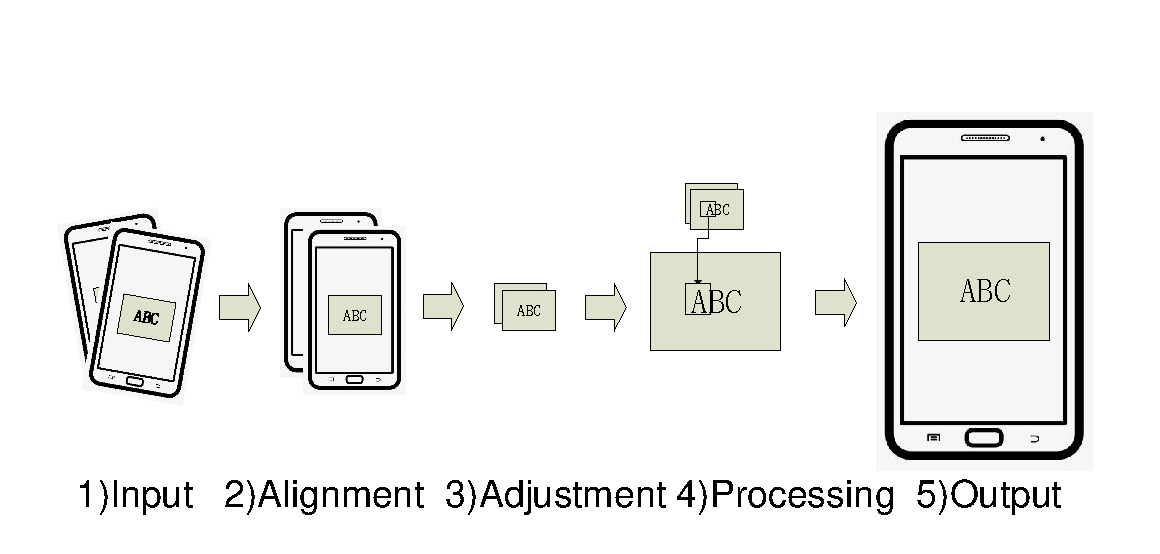
\includegraphics[width=0.5\textwidth]{./pic/workflow.pdf}
       \caption{Illustration of the workflow of our shoulder-surfing system.}
       \label{fig-workflow}
\end{figure}

The outline of this network is as follows:
\begin{itemize}[leftmargin=*]
  \item \textbf{Layered architecture and frequent introduction of input.} To counter the blurriness of the images, and the tendency of reconstructing fake characters, our network is constructed with several identical SR layers, connected sequentially, and the images are refined step by step throughout the layers. The input and output of each layer is also correspondent to each avaliable image\cl{???}, as all input images are processed simultaneously and separately(with the information from other images for reference) throughout the network, all the way to the end of the model where we merge all the data into one output image. Another importent feature of our architecture is that the initial input images are introduced into the dataflow at each layer, from beginning to end, resulting in the uneven depth of our model, acting as an anchor for the reconstruction process so that the output will be faithful to truth from beginning to end, while preserving the deep mainstream of the model to be able to process such blurry images.
  \item \textbf{Merging layers to adapt multiple frames.} The SR layer consists of several convolutional layers and a specially designed merging layer, which is the sole revenue of communication across images. As mentioned above, these images are processed individually thouroughout the network, and they are inputted from the last layer independently, convolutioned independently, and passed to the next layer independently. This apparently cannot fully utilize the information across the multiple frames, so that we design a merging process inside each SR layer, which merges featuremaps from all the images into one, and this data is distributed to each image in this layer and stacked with their featuremaps for the next convolution. In this way, during the refinement process of each of the images in every SR layer, the model has access to data of consensuses among other contemporary images, which can inspire the network to extract more prominent and collective features, and induce the convergence of all input images for increased seamlessness at the successing merging layer. In most deep learning architectures, the features extracted in each layer is more complex than the previous ones, the former's discoveries built on what the latter has achieved, and our model is not an exception; However, the merging layers we designed can support this increase. At each layer the image is exposed to the consensuses of features from other images at the same level of complexity, acting as a verification for the hypothetical features extracted from the current image, so that in the training process more audacious features can be learned and proposed without fear of punishment from the final loss, increasing the quality of featuremaps throughout the network.
  \item \textbf{Model Complexity and adaption for variable input.} All the convolutional layers throughout the network are thus designed: They are performed individually for each image(or the featuremaps of them from the previous layer), and these convolutions in the same layer share a same set of parameters in training and production, thus reducing parameter count and avoiding convolutions for large numbers of channels, saving calculation power. This also leads to the benefit that the output featuremaps of all the images are the evaluations over the same set of features\cl{???}, so that the merging process can also be accomplished easily without the need of trainable parameters. In our design, the merging layers consists of simple pixelwize processes resembling average, min and max processors, to filter out either the collective or the most prominent features among the featuremaps. This process functions with any number of input images. As the convolutional processes are also performed individually for each layer, the same set of parameters of the network model can function normally with any number of input images, while the calculation complexity also increases linearly with the amount of input. On one hand, this gives our model the ability to adapt to the uncertainty of the number of avaliable images, providing relatively satisfactory results regardless whether the attacker has ample time photographing the target phone before it changes its display; on the other hand, the relative independence and the isotropy of the merging layers avoids the reliance on sequential order and consistency between neighboring frames(which is common among most multi-frame SR networks), solving the inconsistency problem mentioned in Figure~\ref{illustration_of_system}.
  \item \textbf{Compatibility with complex characters.} The discrete distribution of characters leads to the inclination of diviation and producing 'fake' results. The frequent introduction of input images is designed to mitigate this challenge. Also, our model is trained on these characters---the images we collected for the training dataset are all cropped so that only the characters remain, so that during the training processes the model can learn correlations between certain features and strokes, and the regular patterns of the characters, narrowing the possibilities offered by the blurry images. We also introduce adaptive boosting\cite{adaboost} in our training process, increasing the loss weight of the wrongly reconstructed characters, determined by loss in earlier stages and OCR in later stages, to accommodate the imbalanceness of data. The loss functions in training is also redesigned. The mean square error(MSE) is not suitable in this application, as a misplaced stroke, although highly obstructing readability, may only invoke a slight decrease in MSE because it only influenced a few pixels. Our solution is putting a weight on each pixel before applying weighted MSE. Assuming the characters are black on white, this weight increases at darker pixels and propagates to neighbouring dark pixels so that long strokes and intersections of strokes are given higher weights. This process serves as a supplement to MSE to focus more on readability and is beneficial for OCR and human reading tests. 
\end{itemize}